\chapter{Generalisation and Optimisation}
\section{Problem statement}
In chapter 2 we saw how to solve an ILP with a CCS matrix using the shortest path framework. Here we want to extend this method to non-CCS matrices and hence create a more general notion of solving ILPs. First this generalisation will yield a solving technique for general matrices over the neutral numbers and later will be further generalized to matrices over the whole numbers who's column sums are strictly positive. 

This generalisation will be done by converting a non-CCS ILP to an equivalent CCS ILP. But this step involves a non-trivial degree of freedom. We will understand and use it, to translate between the equivalent ILPs in such a way, that the shortest path algorithm can be accelerated. 

\section{Converting natural CCS matrices to natural non-CCS matrices}
Our job is to convert non-CCS ILPs into CCS ILPs. But we need to do this in such a way that their solution does not change. For this we can have a look at the underlying system of linear equations $A\vec x = \vec b$. It would be nice to be able to convert any non-CCS $A$ into a CCS $A'$ and maybe also change $\vec b$ to some $\vec b'$ without changing the solution space, namely $\solspace(A;\vec b) = \solspace(A';\vec b')$. But as seen in the lemma \ref{lemma:ilp_pre1}, the solutions of CCS linear systems have a special property, namely that the component sum of all their solutions is constant. This is not true in general. Consider the system of linear equations:
$$
\left(\begin{matrix}
    1 & 2\\
    1 & 2
\end{matrix}\right)
x = \left(\begin{matrix}
    2\\2
\end{matrix}\right)
$$
It yields, amongst others, the solutions $\vec x_1 = (2, 0)^\top$ and $\vec x_2 = (0, 1)^\top$. The component sum of $\vec x_1$ is 2 while the component sum of $\vec x_2$ is 1, which is not equal. This means that we have to accept that we must do a bit of adjustment to the solution space. In the theorem \ref{theorem:column_sum_construction} we will achieve this by adding another component to the solution and thus adding a column to $A$. This first increases the degree of freedom and thus the number of solutions. To capture this increase in the size of the solution space, we will add another row to $A$, i.e. another constraint equation.

Before we dive into the construction, we need a definition to capture matrices without zero columns. In our context of natural numbers, this is equivalent to requiring that the columns all sum to a strictly positive number. As this concept will be useful later, beyond the scope of natural matrices, we will extend the definition \ref{def:CCS} in this way.

\begin{definition}
    \label{def:PCS}
    Let $R$ be an ordered semiring and $\alpha \in R$. Let $S_{>\alpha}(R^{m \times n})$ be the set of matrices of size $m \times n$, who's column all sum up to some number greater then $\alpha$, namely:
    $$S_{>\alpha}(R^{m \times n}) := \{A \in R^{m \times n}\mid \forall j \in [n]\colon \sum_{i=1}^{m} A_{ij} > \alpha\}$$
    For $\alpha = 0$, we will call these matrices \textbf{PCS matrices}, for \textbf{P}ositive \textbf{C}olumn \textbf{S}um.
\end{definition}

Thus natural PCS matrices are exactly those with constant column sum. Now we are ready to tackle the translation of a non-CCM ILP to a CCM ILP.

\begin{theorem}
    \label{theorem:column_sum_construction}
    Let $A\in S_{>0}(\N^{m \times n})$ and $\vec b \in \N^m$. Then, there exists $A' \in S_\alpha(\N^{(m+1) \times (n+1)}), \alpha > 0$ and $\vec b' \in \N^{m+1}$ such that for every $\vec x \in \N^n$:
    $$A\vec x = \vec b \Leftrightarrow \exists x_{n+1}\in \N\colon A' \smat{
        x_1\\
        \vdots\\
        x_n\\
        x_{n+1}
    } = \vec b'$$
\end{theorem}

\begin{proof}
    First we need to get an upper bound in the solutions $\vec x \in \N^n$ in $A\vec x=\vec b$. We will do that similarly as in the proof of lemma \ref{lemma:ilp_pre1}. Let $s_j = \sum_{i=0}^{m} A_{ij}$, the column sum of the $j$-th column in $A$. Let $s := \min\{s_1, \dots, s_j\}$. Because $A$ has no zero-columns $s > 0$.
    $$\sum_{i=1}^m b_i = \sum_{i=1}^{m}\sum_{j=1}^{n}A_{ij} x_j = \sum_{j=1}^{n}\underbrace{\sum_{i=1}^{m}A_{ij}}_{s_j} x_j \geq s \cdot \sum_{j=1}^{n}x_j \Leftrightarrow \sum_{j=1}^{n}x_j \leq \frac{1}{s}\sum_{i=1}^{m}b_i$$
    Now we can construct $A'$ and $\vec b'$. Let $\alpha \geq \max\{s_1, \dots, s_n\}$ and $v_j := \alpha - s_j$. 
    $$A' :=
    \begin{pNiceArray}{cccc}[margin] 
    \Block[draw]{3-3}{A} & & & 0 \\
    & & & \vdots\\
    & & & 0\\
    v_1 & \dots  & v_n & \alpha 
    \end{pNiceArray} \in \N^{(m+1) \times (n+1)}
    \qquad \vec b' := \mat{b_1\\\vdots\\b_m\\\beta} \in \N^{m+1}$$
    It is clear that in $A'$, all columns sum up to $\alpha$. Observe also that $s \leq \alpha$. Because of Lemma \ref{lemma:ilp_pre1} (2) we need to set $\beta := k \cdot \alpha - \sum_{i=0}^{m}b_i$ for some $k \in \N$. We will set $k \geq \frac{1}{s}\sum_{i=1}^{m}b_i$. Thus we get $\beta \geq \frac{\alpha}{s}\sum_{i=1}^{m}b_i - \sum_{i=1}^{m}b_i \geq 0$, because $\frac{\alpha}{s} \geq 1$, which is needed, as $\beta \in \N$. Now we have to prove the equivalence:
    \begin{itemize}
        \item[``$\Leftarrow$''] Because the first $m$ rows in $A'\vec x=\vec b'$ are equivalent to $A\vec x=\vec b$ discarding the last component of the solution $x_{n+1}$ we see that the vector $(x_1, \dots, x_n)^\top$ is indeed a solution to $A\vec x=\vec b$.
        \item[``$\Rightarrow$''] Let $(x_1, \dots, x_n)$ be the solution of $A\vec x=\vec b$. We we have to find a $x_{n+1} \in \N$ such that $\vec x' := (x_1, \dots, x_{n+1})$ is a solution to $A'\vec x' = \vec b'$. 
        
        Now we'll call $(x_1, \dots, x_{n+1}) =: \vec x'$. Because of Lemma \ref{lemma:ilp_pre1} (1) we need to set $x_{n+1} := k - \sum_{j=1}^{n}x_j$. Similarly to the discussion on $\beta$, we also have to make sure for $x_{n+1}$, that it is $\geq 0$. $x_{n+1} \geq k - \frac{1}{s}\sum_{i=1}^{m}b_i \geq \frac{1}{s}\sum_{i=1}^{m}b_i - \frac{1}{s}\sum_{i=1}^{m}b_i = 0$.
        
        Now, we need to check whether $A'\vec x'\stackrel{?}{=}\vec b'$. Because the first $m$ rows in $A'\vec x'=\vec b'$ are equivalent to $A\vec x=\vec b$ discarding the last component of the solution $x_{n+1}$ we only have to check the last row. So we have to prove $(A'\vec x')_{n+1} = \beta$
        \begin{align*}
            (A'x')_{n+1} &= \sum_{j=1}^{n}v_jx_j + \alpha \cdot x_{n+1} = \sum_{j=1}^{n}(\alpha - s_j)x_j + \alpha \cdot x_{n+1} = \alpha \cdot \sum_{j=1}^{n}x_j - \sum_{j=1}^{n}s_jx_j + \alpha \cdot x_{n+1}\\
            &= \alpha \cdot \underbrace{\left(\sum_{j=1}^{n}x_j + x_{n+1}\right)}_k - \sum_{j=1}^{n}s_jx_j = \alpha \cdot k - \sum_{j=1}^{n}\sum_{i=1}^{m}A_{ij}x_j = \alpha\cdot k - \sum_{i=1}^{m}\underbrace{\sum_{j=1}^{n}A_{ij}x_j}_{b_i}\\
            &= \alpha\cdot k - \sum_{i=1}^{m}b_i = \beta &&\qedhere
        \end{align*}
    \end{itemize}
\end{proof}
With this construction in our belts, we can take any PCS ILP and convert it to a CCS ILP and solve it using the shortest path framework. But this conversion may not be great and we can improve it, which will result in smaller graphs.

\section{Optimising the conversion}
\subsection{Introductory example}
In the last chapter we saw that the speed of solving ILPs in the manner of a shortest path problem is strongly influenced by the number of layers in the corresponding graph. We called this number $k$ and it is equal to the sum of the components of the solutions of $A\vec x=\vec b$. We needed the columns of $A$ to all sum to the same number. If $A$ did not have this property, we could construct a new matrix $A'$ that had this property and minimally changed the solution space. For this we used the theorem \ref{theorem:column_sum_construction}, where we were able to choose some $k$, which again drastically affects the runtime of the algorithm. There we had to put a restriction on $k$, namely
$$k \geq \frac{1}{\min_{j \in [n]} \left\{ \sum_{i=1}^{m}A_{ij}\right\}}\cdot \sum_{i=1}^{m}b_i$$
You may observe that equivalent linear systems of equations might produce different bounds. Let us look at the following simple example. We want to solve 
$$\mat{1&2\\0&6}\vec x = \mat{7\\18} \qquad \Rightarrow k \geq \frac{7 + 18}{\min\{1+0, 2+6\}} = 25$$
Meaning if we would solve an ILP with this system of linear equations we would need a graph with 25 layers. Now let us modify this system by multiplying the first row by 100:
$$\mat{100&200\\0&6}\vec x = \mat{700\\18} \qquad \Rightarrow k \geq \frac{700 + 18}{\min\{100+0, 200+6\}} = \frac{718}{100} \Rightarrow k \geq 8$$
We have achieved a major reduction of the number of layers and thus dramatically shrank the graph. In the following arguments we explore these kinds of manipulations and discover a strategy on how you would systematically minimizing $k$. But first, we have to understand the behavior better.

\subsection{Getting a grip: Define a cost function}
Lets first define a few helpful functions. Let $k\colon S_{>0}(\N^{m \times n}) \times \N^m \to \R$ be
$$k(A, \vec b) := \frac{1}{\min_{j \in [n]} \left\{ \sum_{i=1}^{m}A_{ij}\right\}}\cdot \sum_{i=1}^{m}b_i$$
So we need to find a $k \geq k(A, \vec b)$. Since $k(A, \vec b)$ determines how many layers the resulting graph will have, we can think of it as a kind of cost function. Now we are going to generalise this cost function. But how do we do that? The goal is to perform very specific Gauss manipulations on $A\vec x = \vec b$. But not all values of the resulting system of equations are interesting for $k$, only the column sums in $A$ and the component sums in $\vec b$. To figure this out, all we need to keep track of is how much each row has been scaled up or down, in other words, how much it contributes to the resulting system of equations. To keep track of this, we store these values in a vector $\vec\mu$, where $\mu_i$ indicates how much the $i$-th row has been scaled up. The vector $\opvec(1)$, which consists only of ones, thus represents the original matrix, since each row has not been scaled (i.e. scaled by 1). Finding the column sum in the $j$-th column after the transformation is the standard dot product of the $j$-th column $\vec a_j$ and $\vec\mu$. For example, with $\vec \mu = \opvec(1)$, $\sprod{\vec a_j}{\opvec(1)}$ is really just the $j$-th column sum in the original $A$. Hence, we will generalize $k(A, \vec b)$ as follows:
$$k(A, \vec b; \vec \mu) := \frac{\sprod{\vec{\mu}}{\vec b}}{\min_{j \in [m]} \sprod{\vec \mu}{\vec a_j}}$$
where $\vec a_j$ is the $j$-th column of $A$. Because we want the columns sum to always stay positive after the transformation we want to restrict $\vec\mu$ to those values where for all column $\vec a_j$ hold that $\sprod{\vec a_j}{\vec\mu} > 0$. More formally: we restrict $\vec\mu$ to:
$$\vec \mu \in U_A := \{\vec x \in \R^m \mid \forall j \in [m]\colon \sprod{\vec x}{\vec a_j} > 0\}$$
Note that because all entries of $A$ are non-negative, $U_A$ is a superset of $\R_{>0}^m$. We also see that $k(A, \vec b) = k(A, \vec b; \opvec(1))$, where $\opvec(1) = (1, \dots, 1)^\top$. And also $\opvec(1) \in U_A$, because $\opvec(1) \in \R^m_{>0}$. It is left to show, why exactly this generalization is as useful as promised. This will be handled by the next lemma:
\begin{lemma}
    \label{lemma:construct_gauss_steps}
    Let $A \in S_{>0}(\N^{m \times n}), \vec b \in \N^m$. Then the following to statements will hold:
    \begin{enumerate}
        \item[1)] $\forall \vec \mu \in U_A \cap \Q^m$ exist $A' \in \N^{m \times n}, \vec b' \in \N^m$, such that $\solspace(A, \vec b) = \solspace(A', \vec b')$ and
        $k(A', \vec b') = k(A, \vec b; \vec\mu)$
        \item[2)] $\forall  A' \in \N^{m \times n}, \vec b' \in \N^m$, such that $\solspace(A, \vec b) = \solspace(A', \vec b')$ exists a $\vec \mu \in U_A \cap \Q^m$, such that 
        $k(A', \vec b') = k(A, \vec b; \vec\mu)$.
    \end{enumerate}
\end{lemma}
\begin{proof}
    \begin{enumerate}
        \item[1)] Because $k(A, \vec b; \vec \mu) = k(A, \vec b; \lambda \vec \mu)$ for $\lambda > 0$ we can w.l.o.g. assume that $\vec \mu \in \Z^m$. Because we need to construct $A'$ and $\vec b'$ such that $\solspace(A, \vec b) = \solspace(A', \vec b')$ there must exist a $C \in \GL_m(\Q)$ such that $A' = C\cdot A$ and $\vec b = C\cdot \vec b$. Thus it suffices to construct $C$. So the task will be to select $C$ such that
        $$C^\top \cdot \opvec(1) = \lambda \vec\mu, \quad A' = C\cdot A \in \N^{m \times n} \quad \textrm{and} \quad \det(C) \neq 0$$
        for some $\lambda \in \N \setminus \{0\}$. Then it will hold that:
        \begin{align*}
            k(A', \vec b') &= k(A', \vec b'; \opvec(1)) = k(C \cdot A, C \cdot \vec b; \opvec(1))\\
            &= \frac{\sprod{\opvec(1)}{C \cdot \vec b}}{\min_{j \in [m]} \sprod{\opvec(1)}{C \cdot \vec a_j}} = \frac{\sprod{C^\top \cdot \opvec(1)}{\vec b}}{\min_{j \in [m]} \sprod{C^\top \cdot \opvec(1)}{\vec a_j}}\\
            &= \frac{\sprod{\lambda\vec{\mu}}{\vec b}}{\min_{j \in [m]} \sprod{\lambda\vec \mu}{\vec a_j}} = k(A, \vec b; \lambda\vec\mu) \stackrel{\checkmark}{=} k(A, \vec b; \vec\mu)
        \end{align*}
        How do we actually find that $C$. We will split that task into 2 tasks, by constructing 2 matrices $C', D  \in \GL_m(\Z)$, setting $C := C' \cdot D$ with the properties:
        \begin{itemize}
            \item $C'^\top \cdot \opvec(1) = \lambda \cdot \opvec(1)$
            \item $D^\top \cdot \opvec(1) = \vec\mu$
            \item $A' = C' \cdot D\cdot A$ has only non-negative entries
        \end{itemize}
        In other words: $D$ will make sure that each row does actually contribute as much as specified in $\vec\mu$ to the transformed system of linear equations and $C'$ makes sure that all entries in $A'$ are positive.

        If we can find such $C', D$ we are done, because $\det(C) \neq 0$ and $ A' = C\cdot A \in \N^{m \times n}$ is clear and $C^\top \cdot \opvec(1) = D^\top \cdot C'^\top\cdot \opvec(1) = \lambda \cdot D^\top \opvec(1) \stackrel{\checkmark}{=}\lambda\vec\mu$. So let us do it one by one:

        $$D := \mat{
            d_1 & e_2 & 0 & \dots & 0 & 0\\
            0 & d_2 & e_3 & \dots & 0 & 0\\
            0 & 0 & d_3 & \dots & 0 & 0\\
            \vdots & \vdots & \vdots & \ddots & \vdots & \vdots\\
            0 & 0 & 0 & \dots & d_{m-1} & e_m\\
            e_1 & 0 & 0 & \dots & 0 & d_m
        } \quad\textrm{with}\quad 
        \begin{matrix}
            d_i := \begin{cases}
                \mu_i &\textrm{if}\quad \mu_i \neq 0\\
                1 &\textrm{if}\quad \mu_i = 0
            \end{cases}\\\\
            e_i := \begin{cases}
                0 &\textrm{if}\quad \mu_i \neq 0\\
                -1 &\textrm{if}\quad \mu_i = 0
            \end{cases}
        \end{matrix}$$
        we see that $(D^\top \cdot \opvec(1))_i = d_i + e_i \stackrel{\checkmark}{=} \mu_i$. We still have to make sure that $D$ is invertible, meaning $\det(D) \neq 0$. Let us compute the determinant by applying laplace expansion to the first column. We get:
        \begin{align*}  
            \det(D) &= d_1 \cdot \det\mat{
                d_2 & e_3 & \dots & 0 & 0\\
                0 & d_3 & \dots & 0 & 0\\
                \vdots & \vdots & \ddots & \vdots& \vdots\\
                0 & 0 & \dots & d_{m-1} & e_m\\
                0 & 0 & \dots & 0 & d_m
            } \pm e_1 \cdot \det\mat{
                e_2 & 0 & \dots & 0 & 0\\
                d_2 & e_3 & \dots & 0 & 0\\
                \vdots & \vdots & \ddots & \vdots& \vdots\\
                0 & 0 & \dots & e_{m-1} & 0\\
                0 & 0 & \dots & d_{m-1} & e_m
            }\\
            &= d_1 \cdot d_2 \cdot d_3 \cdot ... \cdot d_m \pm e_1 \cdot e_2 \cdot e_3 \cdot ... \cdot e_m 
        \end{align*}
        Because $\vec\mu \neq \vec0$, we know that at least one $e_i$ must be 0. Thus $e_1 \cdot e_2 \cdot e_3 \cdot ... \cdot e_m = 0 \Rightarrow \det(D) = d_1 \cdot d_2 \cdot d_3 \cdot ... \cdot d_m \neq 0$.

        Now we construct $C'$. For that let $\tilde A := D \cdot A$ and $c := \max_{i \in [m], j\in[n]} |\tilde A_{ij}| > 0$ the largest absolute value in $\tilde A$. Let $\opmat_m(c) \in \N^{m\times m}$ be the matrix, with only $c$ as entries. Then we can choose $C'$:
        $$C' := \imat_m + \opmat_m(c)$$
        It is easy to see, that $C'^\top \opvec(1) = \imat_m\cdot \opvec(1) + \opmat_m(c)\cdot \opvec(1) = \opvec(1) + mc \opvec(1) = (1 + mc)\opvec(1)$. So the necessary property holds, with $\lambda = mc+1$. We have to check again, that $C'$ is indeed invertible. Let us assume there exists a vector $\vec v \in \Q^m, \vec v \neq \vec0$ such that $C'\vec v = \vec 0 \Leftrightarrow \vec0 = \vec v + \opmat_m(c)\vec v \Leftrightarrow \opmat_m(c)\vec v = -\vec v$. For that to be true, $\opmat_m(c)$ must have the eigenvalue $-1$. It is easy to guess all $m$ eigenvalues of $\opmat_m(c)$: eigenvector $\opvec(1)$ yields the eigenvalue $cm>0$ and the family of vectors in the shape $(1, 0, \dots, 0, -1, 0, \dots, 0)$ yield $m-1$ eigenvalues of value $0$. Thus $-1$ is not an eigenvalue of $\opmat_m(c)$ and $\vec v$ does not exist and $C'$ is invertible.

        The last step is making sure, that $A'$ only contains non-negative entries. Remember that $\tilde A = D \cdot A$, thus $A' = C' \cdot \tilde A$. We see that $(\tilde A^\top \opvec(1))_j =(A^\top\cdot D^\top\cdot \opvec(1))_j = (A^\top \vec\mu)_j = \sprod{\vec a_j}{\vec\mu} > 0$. But because all numbers involved are whole numbers, we even further now that $(\tilde A^\top \opvec(1))_j \geq 1$. Now let us check the non-negativity of $A'$:

        \begin{align*}
            A'_{ij} &= (C'\cdot \tilde A)_{ij} = (\imat_m \cdot \tilde A)_{ij} + (\opmat_m(c)\cdot \tilde A)_{ij}\\
            &= \tilde A_{ij} + \sum_{k=1}^{m}\opmat_m(c)_{ik} \tilde A_{kj} = \tilde A_{ij} + c \cdot \sum_{k=1}^{m} \tilde A_{kj} = \tilde A_{ij} + c \cdot (\tilde A^\top \opvec(1))_j\\
            &\geq \tilde A_{ij} + c \geq - |\tilde A_{ij}| + c \geq - c + c = 0
        \end{align*}
        
        \item[2)] Because $\solspace(A, \vec b) = \solspace(A', \vec b')$, there must exist a $C \in \GL_m(\Q)$, such that $A' = C \cdot A \in \N^{m \times n}$ and $\vec b' = C \cdot \vec b \in \N^m$. As in 1) we will choose $\vec \mu := C^\top \cdot \opvec(1)$ and thus:
        \begin{align*}
            k(A, \vec b; \vec\mu) &= \frac{\sprod{\vec\mu}{\vec b}}{\min_{j\in [m]}\sprod{\vec\mu}{\vec a_j}} = \frac{\sprod{C^\top\cdot\opvec(1)}{\vec b}}{\min_{j\in [m]}\sprod{C^\top\cdot\opvec(1)}{\vec a_j}}\\
            &= \frac{\sprod{\opvec(1)}{C\cdot\vec b}}{\min_{j\in [m]}\sprod{\opvec(1)}{C\cdot\vec a_j}} = k(C\cdot A, C\cdot\vec b; \opvec(1)) \stackrel{\checkmark}{=} k(A', \vec b')
        \end{align*}
        It is left to check whether $\vec \mu \in U_A$. Because $A$ had no zero columns, $A'$ also has none, which means that for every $j \in [m]$:
        \begin{equation*}
            0 < \sprod{\opvec(1)}{\vec a'_j} = \sprod{\opvec(1)}{C \cdot \vec a_j} = \sprod{C^\top \cdot \opvec(1)}{\vec a_j} = \sprod{\vec \mu}{\vec a_j} \qquad \Rightarrow\vec \mu \in U_A \qedhere
        \end{equation*}

    \end{enumerate}
\end{proof}

Statement 2) says that for any other equivalent system of equations we find a $\vec \mu$ that represents it. And 1) states the reverse, i.e. that for every $\vec \mu$ we find a corresponding system of equations. This means that all equivalent systems of equation are exactly covered by the function $k(A, \vec b; \vec\mu)$ for some $\vec \mu$. This means, for finding the optimal $k$ we just need to minimize $k(A, \vec b; \vec \mu)$ over $\vec \mu$.

Before we proceed, one last note about continuity. Because $k(A, \vec b; \vec \mu)$ is continuous when changing $\vec\mu$, we will find for every $\varepsilon > 0$ and $\vec\mu \in U_A$ a $\vec\mu' \in U_A \cap \Q^m$ such that $|k(A, \vec b; \vec \mu) - k(A, \vec b; \vec \mu')| < \varepsilon$. This means all further discussions can be done in $\R^m$. Conveniently, the minima we will be finding are actually all in $\Q^m$.

Let us simplify notation. We will now consider $A \in \N^{m \times n}$ and $\vec b \in \N^m$ as given. And we will write $k(\vec \mu) := k(A, \vec b; \vec \mu)$ and also $U := U_A$. Our goal is to minimize $k(\vec \mu)$ over $U$.

By 2 simple observation we can already make a lot of progress. Note that $\delta U = \{\vec x \in \R^m \mid \min_{j \in [n]}\sprod{\vec x}{\vec a_j} = 0\}$ and thus $k(\vec \mu)$ blows up to infinity when $\vec \mu \to \delta U$. Hence the minimum we are seeking cannot lie on the border of $U$. Furthermore note that $k(\vec \mu) = k(\lambda \vec\mu)$ for any $\lambda > 0$. This means that $k(\vec \mu)$ will have the same value along a ray starting at the origin. Thus it is sufficient to only consider a $m-1$-dimensional surface of a sphere, which is compact. Remember that any continuous function on will attain its maximum and minimum at least once on a compact set. Therefore we know, that any minima that will be reached are local minima in $U$.

Because we now know that we are only interested in local minima in $U$, we can start analyzing $k(\vec \mu)$ a little bit closer. But first, more notation:
$$U_j := \{\vec x \in U \mid \forall j' \in [n]\colon \sprod{\vec x}{\vec a_j} \leq \sprod{\vec x}{\vec a_{j'}}\} \subseteq U$$
$U_j$ is thus the area where $\sprod{\vec\mu}{\vec a_j}$ is the smallest dot product and hence:
$$\restrict{k(\vec\mu)}{U_j} = \frac{\sprod{\vec\mu}{\vec b}}{\sprod{\vec\mu}{\vec a_j}}$$
Especially interesting are those areas, where different $U_j$'s meet. This can be seen in the next lemma:

\begin{lemma}
    \label{lemma:k_behavior}
    Let $\vec a_1, \dots, \vec a_n \in \N^m \setminus \{\vec0\}$, $U_j := \{\vec x \in \R^m \mid \forall j' \in [n]\colon \sprod{\vec x}{\vec a_j} \leq \sprod{\vec x}{\vec a_{j'}}\}$ and $k(\vec \mu) := \frac{\sprod{\vec{\mu}}{\vec b}}{\min_{j \in [m]} \sprod{\vec \mu}{\vec a_j}}$. Let $j_1, \dots, j_r \in [n]$ a selection of indices, such that $U_{j_1} \cap \dots \cap U_{j_r} \neq \emptyset$.  Then it will hold that:
    \begin{itemize}
        \item[1)] $\vec b \in \Span(\vec a_{j_1}, \dots, \vec a_{j_r}) \Rightarrow \restrict{k(\vec \mu)}{U_{j_1} \cap \dots \cap U_{j_r}}$ is constant.
        \item[2)] $\vec b \notin \Span(\vec a_{j_1}, \dots, \vec a_{j_r}) \Rightarrow \restrict{k(\vec \mu)}{U_{j_1} \cap \dots \cap U_{j_r}}$ is strictly monotone.
    \end{itemize}
\end{lemma}
\begin{proof}
    Because $\vec \mu \in U_{j_1}\cap \dots\cap U_{j_r}$ the following 2 statements will hold:
    $$\sprod{\vec{\mu}}{\vec a_{j_1}} = \dots = \sprod{\vec{\mu}}{\vec a_{j_r}} \quad\textrm{and}\quad k(\vec\mu) = \frac{\sprod{\vec \mu}{\vec b}}{\sprod{\vec \mu}{\vec a_{j_1}}}$$
    Now let us consider the two cases separately\\
    \textbf{Case 1} $\vec b \in \Span(\vec a_{j_1}, \dots, \vec a_{j_r}) \Rightarrow\exists c_1, \dots, c_r \in \R\colon \vec b = c_1\vec a_{j_1} + \dots + c_1\vec a_{j_r}$.
    $$k(\vec\mu) = \frac{\sprod{\vec \mu}{\vec b}}{\sprod{\vec \mu}{\vec a_{j_1}}} = c_1 \cdot \underbrace{\frac{\sprod{\vec \mu}{\vec a_{j_1}}}{\sprod{\vec \mu}{\vec a_{j_1}}}}_1 + \dots + c_r \cdot \underbrace{\frac{\sprod{\vec \mu}{\vec a_{j_r}}}{\sprod{\vec \mu}{\vec a_{j_1}}}}_1 = c_1 + \dots + c_r \quad \Rightarrow k(\vec\mu)\textrm{ is constant}$$
    \textbf{Case 2} $\vec b \notin \Span(\vec a_{j_1}, \dots, \vec a_{j_r}) \Rightarrow\lnot\exists c_1, \dots, c_r \in \R\colon \vec b = c_1\vec a_{j_1} + \dots + c_1\vec a_{j_r}$. We want to optimize a function subject to some constraints. For that, we will be using the method of Lagrange multipliers. We have $r-1$ constraints of the following shape:
    $$\sprod{\vec\mu}{\vec a_{j_l}} = \sprod{\vec\mu}{\vec a_{j_{l+1}}} \Leftrightarrow \sprod{\vec\mu}{\vec a_{j_l} - \vec a_{j_{l+1}}} = 0, \quad l \in [r-1]$$
    Thus we get the Lagrangian
    \begin{align*}
        \lagrangian(\vec\mu, \lambda_1, \dots, \lambda_{r-1}) &= \frac{\sprod{\vec \mu}{\vec b}}{\sprod{\vec \mu}{\vec a_{j_1}}} - \sum_{l=1}^{r-1}\lambda_l \sprod{\vec\mu}{\vec a_{j_l} - \vec a_{j_{l+1}}}\\
        \vec0 \stackrel{!}{=}\nabla_{\vec \mu} \lagrangian(\vec\mu, \lambda_1, \dots, \lambda_{r-1}) &= \frac{\vec b\sprod{\vec\mu}{\vec a_{j_{1}}} - \sprod{\vec\mu}{\vec b}\vec a_{j_{1}}}{\sprod{\vec\mu}{\vec a_{j_{1}}}^2} - \sum_{l=1}^{r-1}\lambda_l(\vec a_{j_l} - \vec a_{j_{l+1}}) \\
        \Rightarrow\quad \vec0 &= \vec b\sprod{\vec\mu}{\vec a_{j_{1}}} - \sprod{\vec\mu}{\vec b}\vec a_{j_{1}} - \sprod{\vec\mu}{\vec a_{j_{1}}}^2\cdot\sum_{l=1}^{r-1}\lambda_l(\vec a_{j_l} - \vec a_{j_{l+1}})\\
        \Rightarrow\quad \vec b &= \frac{\sprod{\vec \mu}{\vec b}}{\sprod{\vec \mu}{\vec a_{j_{1}}}}\vec a_{j_{1}} + \sum_{l=1}^{r-1} \lambda_r \sprod{\vec\mu}{\vec a_{j_{1}}}(\vec a_{j_l} - \vec a_{j_{l+1}})
    \end{align*}
    This is just a linear combination of $\vec a_{j_1}, \dots \vec a_{j_r}$, which we forbid in the first place. Thus this also yields a contradiction meaning that $k(\vec\mu)$ is strictly monotone.
\end{proof}

A local minimum can only be attained when the gradient vanishes. Because of the last lemma, I only need to find different sets of $\{\vec a_{j_1}, \dots, \vec a_{j_r}\} \subseteq \{\vec a_1, \dots, \vec a_n\}$ such that $\vec b \in \Span(\vec a_{j_1}, \dots, \vec a_{j_r})$ and $U_{j_1} \cap \dots \cap U_{j_r} \neq \emptyset$ and then compare their $k(\vec\mu)$ for some $\vec\mu \in U_{j_1} \cap \dots \cap U_{j_r}$. The right selection of $\{\vec a_{j_1}, \dots, \vec a_{j_r}\}$ will be key in understanding the minimization of $k(\vec\mu)$. 

\subsection{Minimizing the cost function}
Now we need to find a $\vec\mu$ that minimizes $k(\vec\mu)$. I will now give a rough outline of how to find the correct $\mu$, leaving out the details. But it will be enough to show the correctness of this approach. Then I will fill in the details of how to do each step efficiently. But first, a definition:
\begin{definition}
    Let $M \in \N^{m\times n}$ be a matrix. Then $\Delta(M) \in \Z^{(n-1)\times m}$ is also a matrix such that 
    $$\Delta(M)_{i,j} = M_{j,i} - M_{j,i+1}$$
\end{definition}
\begin{observation}
    \label{obs:delta_meaning}
    This is useful, as all $\vec x$ solving $\Delta(M)\vec x = \vec 0$ will have the property that all columns of $M$ (let they be $\vec m_1, \dots, \vec m_n$) yield the same dot-product with $\vec x$, in other words $\sprod{\vec x}{\vec m_1} = \dots = \sprod{\vec x}{\vec m_n}$.
\end{observation}

Now let us describe the outline for the algorithm. It mainly involves two steps:
\begin{algorithm}
    \label{algo}
    \begin{enumerate}
        \item Compute the convex hull of $\vec a_1, \dots, \vec a_n$. Send a ray from the origin to $\vec b$ and record the first facet of the convex hull it collides with. If it hits a lower dimensional facet, we'll take that. Let the vertices of that facet be $\vec a_{j_1}, \dots, \vec a_{j_r}$. Create a new matrix $A' := (\vec a_{j_1}, \dots, \vec a_{j_r}) \in \N^{m \times r}$.
        \item Find a $\vec\mu \in \solspace(\Delta(A'), \vec0) \setminus \solspace(A'^\top, \vec0)$. If $\sprod{\vec\mu}{\vec a_{j_1}}<0$, take $-\vec\mu$ instead. This will yield the minimal value for $k(\vec\mu)$.
    \end{enumerate}
\end{algorithm}

Now we have to answer the question of correctness. And we will do this in several steps. First, we will show that the algorithm always returns a value, then that this value is a local minimum, and finally that this local minimum is the smallest local minimum there is, and thus the global minimum. But first I will define some terms that we will need throughout our journey.
\begin{definition}
    \label{def:algo_basic}
    Let $A \in S_{>0}(\N^{m \times n})$. Let $\vec a_j$ be the $j$-th column of $A$. Let $\vec a_{j_1}, \dots, \vec a_{j_r}$ and $A' \in \N^{m\times r}$ be as in step 1 in the algorithm \ref{algo}. Let $\vec b \in \N^m$ such that $\exists \vec x \in \N^n\colon A\vec x = \vec b$. Let $U := \{\vec\mu \in \R^m\mid \forall j \in [n]\colon\sprod{\vec\mu}{\vec a_j} > 0\}$. Let $U_j := \{\vec\mu \in U \mid \forall j'\in[n]\colon \sprod{\vec\mu}{\vec a_j} \leq \sprod{\vec\mu}{\vec a_{j'}}\}$. Let $k\colon \R^m\to\R$ be defined as 
    $$k(\vec\mu) := \frac{\sprod{\vec\mu}{\vec b}}{\min_{j\in[n]}\sprod{\vec\mu}{\vec a_j}}$$
\end{definition}

\subsubsection{Existance of a result}
First of all, we have to ask ourselves whether the algorithm always produces an output. Step 1 requires that the ray actually intersects the convex hull, while for step 2 $\solspace(\Delta(A'), \vec0) \setminus \solspace(A'^\top, \vec0)$ must not be empty. I will clarify this now:

\begin{lemma}
    \label{lemma:b_behind_hull}
    Let $\vec b, \vec x, \vec a_1, \dots, \vec a_n$ as in definition \ref{def:algo_basic}. Then there exists $\gamma \in \Q$, $0 < \gamma \leq 1$ such that $\gamma \vec b$ lies inside the convex hull of $\vec a_1, \dots, \vec a_n$.
\end{lemma}
\begin{proof}
    By assumption, we know that $\vec b = \sum_{j=1}^{n}x_j \vec a_j$ with $\sum_{j=1}^{n}x_j =: s \geq 1$. Let $\gamma := \frac{1}{s}$, thus $0 < \gamma \leq 1$. Now let us construct $\gamma\vec b$ using $\vec a_1, \dots, \vec a_n$:
    $$\gamma\vec b = \frac{1}{s}\sum_{j=1}^{n}x_j \vec a_j = \sum_{j=1}^{n}\frac{x_j}{s}\vec a_j =: \sum_{j=1}^{n} \lambda_j\vec a_j \qquad \mathrm{with}\quad \sum_{j=1}^{n}\lambda_j = \frac{1}{s}\cdot \sum_{j=1}^{n} x_j = \frac{1}{s}\cdot s = 1, \lambda_j \geq 0$$
    Thus $\gamma\vec b$ is representable as a convex combination of $\vec a_1, \dots, \vec a_n$ and therefore lies in their convex hull.
\end{proof}
This lemma ensures that on the way from the origin to $\vec b$ we will hit the convex hull, which ensures that step 1 will always have a result. We will deal with the non-emptiness of $\solspace(\Delta(A'), \vec0)\setminus \solspace(A'^\top, \vec0)$ in two separate lemmas:

\begin{lemma}
    \label{lemma:visible_facets_are_linearly_independent}
    Let $\vec v_1, \dots, \vec v_n \in \N^m \setminus\{\vec0\}$ and $C := \conv(\vec v_1, \dots, \vec v_n)$ be their convex hull. Let $R = \{\gamma \vec d \mid \gamma \in \R_{\geq 0}\}$ be a ray from the origin and $\vec v_{j_1}, \dots, \vec v_{j_r}$ the corners of the (sub-)facet of $C$, $R$ hits first. Then $\vec v_{j_1}, \dots, \vec v_{j_r}$ are lineally independent. By a (sub-)facet, I mean the lowest dimensional facet that got hit by $R$.
\end{lemma}
\begin{proof}
    I'll show that $\vec 0 \notin \aff(\vec v_{j_1}, \dots, \vec v_{j_r})$ by contradiction which then implies that $\vec v_{j_1}, \dots, \vec v_{j_r}$ are lineally independent, because if not, there exists a linear dependence $\vec 0 = \lambda_1\vec v_{j_1} + \dots + \lambda_r\vec v_{j_r}$ with $\lambda_1 + \dots + \lambda_r = 1 \Rightarrow\exists\lambda_j\colon\lambda_j \neq 0$. 
    
    Let us assume that $\vec 0 \in \aff(\vec v_{j_1}, \dots, \vec v_{j_r})$, thus $\vec 0 = \lambda^{(\vec 0)}_1 \vec v_{j_1} + \dots + \lambda^{(\vec 0)}_r \vec v_{j_r}$ with $\lambda^{(\vec 0)}_1 + \dots + \lambda^{(\vec 0)}_r = 1$. Let $\vec p$ the first intersection of $R$ and the convex hull thus $\vec p = \lambda^{(\vec p)}_1 \vec a_{j_1} + \dots + \lambda^{(\vec p)}_r \vec a_{j_r}$ with $\lambda^{(\vec p)}_1 + \dots + \lambda^{(\vec p)}_r = 1$ and $\lambda^{(\vec p)}_j \geq 0$ Let $\nu \in [0, 1]$. Any point $\nu\vec p$ is also representable as an affine combination, because
    \begin{align*}
        \nu \vec p &= \nu \vec p + (1-\nu)\vec 0 = \nu\lambda^{(\vec p)}_1 \vec v_{j_1} + \dots + \nu\lambda^{(\vec p)}_r \vec v_{j_r} + (1-\nu)\lambda^{(\vec 0)}_1 \vec v_{j_1} + \dots + (1-\nu)\lambda^{(\vec 0)}_r \vec v_{j_r}\\
        &=(\nu\lambda^{(\vec p)}_1 + (1-\nu)\lambda^{(\vec 0)}_1)\vec v_{j_1} + \dots + (\nu\lambda^{(\vec p)}_r + (1-\nu)\lambda^{(\vec 0)}_r)\vec v_{j_r} =: \lambda_1(\nu)\vec v_{j_1} + \dots + \lambda_r(\nu)\vec v_{j_r}
    \end{align*}
    with $\lambda_j(\nu) := \nu\lambda^{(\vec p)}_j + (1-\nu)\lambda^{(\vec 0)}_j$.

    It is easy to see, that $\forall \nu\in[0, 1]: \lambda_1(\nu) + \dots + \lambda_r(\nu) = 1$., hence for every $\nu$ this gives us an affine combination. $\lambda_j(\nu)$ are linear functions, with $\lambda_j(0) = \lambda_j^{(\vec 0)}$ and $\lambda_j(1) = \lambda_j^{(\vec p)}$. Because all $\vec v_j$ have non-negative entries and none of them is $\vec 0$ we know that there must be at least one $\lambda_j^{(\vec 0)}$ that is negative. Because all $\lambda_j^{(\vec p)}$ are non-negative, there must exist at least one function $\lambda_j(\nu)$ that has a zero in $\nu \in [0, 1]$. Let us select the highest zero $\nu_0 := \max\{\nu \in [0, 1]\mid \exists j\in [n]\colon \lambda_j(\nu) = 0\}$. Observe that, if $\nu \geq \nu_0$ that $\nu\vec p \in \conv(\vec v_{j_1}, \dots, \vec v_{j_r})$, because $\forall \nu \geq \nu_0, j\in[n]\colon \lambda_j(\nu) \geq 0$. But $\vec p$ is the first intersection with the convex hull and this forces $\nu_0 = 1$. Well, that means that at least one coefficient in $\lambda^{(\vec p)}_1, \dots, \lambda^{(\vec p)}_r$ is zero. Thus there exists a lower dimensional facet, namely the convex hull of the corners who's coefficients are non-zero. Thus $\vec v_{j_1}, \dots, \vec v_{j_r}$ are not the corners of the lowest dimensional facet possible $\vec p$ lies in, the contradiction.
\end{proof}

\begin{observation}
    \label{obs:hit_facet_is_linearly_independent}
    A direct implication of lemma \ref{lemma:visible_facets_are_linearly_independent} is that the set $\{\vec a_{j_1}, \dots, \vec v_{j_r}\}$, the result of step 1 of the algorithm, is linearly independent.  
\end{observation}

\begin{lemma}
    \label{lemma:solspace_big_enough}
    Let $A'$ be as in definition \ref{def:algo_basic}. Then $\dim(\solspace(\Delta(A'), \vec0)) > \dim(\solspace(A'^\top, \vec0))$.
\end{lemma}
\begin{proof}
    Observe that $\dim(\solspace(\Delta(A'), \vec0)) = \nullity(\Delta(A'))$ and also $\dim(\solspace(A'^\top, \vec0)) = \nullity(A'^\top) =$ $\nullity(A')$. Because of observation \ref{obs:hit_facet_is_linearly_independent} it will hold that $\rank(A') = r$. As $\Delta(A')$ has only $r-1$ rows, $\rank(\Delta(A')) \leq r-1 < r$. Now we can apply the rank-nullity theorem to $A'^\top$ and $\Delta(A')$.
    $$m = \rank(A'^\top) + \nullity(A'^\top) \Leftrightarrow \nullity(A^\top) = m - r$$
    $$m = \rank(\Delta(A')) + \nullity(\Delta(A')) < r + \nullity(\Delta(A'))\Leftrightarrow \nullity(\Delta(A')) > m - r$$
    Combining these two results yields $\nullity(\Delta(A')) > \nullity(A'^\top)$ the result we wanted to show.
\end{proof}
Subtracting a lower dimensional vector space from a bigger dimensional one will always yield some vectors and thus $\solspace(\Delta(A'), \vec0) \setminus \solspace(A'^\top, \vec0)$ is non-empty.

\subsubsection{The result is a local minimum}
We have already seen in the lemma \ref{lemma:k_behavior} that $\restrict{k(\vec\mu)}{U_{j_1}\cap \dots \cap U_{j_r}}$ is constant if and only if $\vec b \in \Span(\vec a_{j_1}, \dots, \vec a_{j_r})$. We can already see that the basis selected in step 1 fulfils these criteria. The next step is to show that the $\vec\mu$ we selected is actually in $U_{j_1} \cap \dots \cap U_{j_r}$. This may be obvious, since by construction $\vec\mu \in \solspace(\Delta(A'), \vec 0)$ and by observation \ref{obs:delta_meaning} it will hold that $\sprod{\vec a_{j_1}}{\vec\mu} = \dots = \sprod{\vec a_{j_r}}{\vec\mu} =: d$. But it is not clear that $d$ is actually the smallest dot product, which is the necessary condition for $U_{j_1}, \dots, U_{j_r}$. We don't even know a priori whether ${U_{j_1} \cap \dots \cap U_{j_r}}$ is not empty. These are the things that will be covered in this section. But before we dive deep into the explanation, I need to make a general observation:

\begin{lemma}
    \label{lemma:affine_space}
    Let $\vec v_1,\dots,\vec v_r$ be a linearly independent set in $\R^n$, and let $H$ be the unique $(r-1)$-dimensional affine space passing through $\vec v_1,\dots,\vec v_r$. Then $H$ separates the $r$-dimensional subspace span$(\vec v_1,\dots,\vec v_r)$ into two open half-spaces: one piece $S_0$ contains the origin and the other piece $S_1$ does not. Furthermore and more crucially: if $\vec p = \sum_{i=1}^r \lambda_i \vec v_i$ is any vector in span$(\vec v_1,\dots,\vec v_r)$, then
    $$
    \sum_{i=1}^r \lambda_i < 1 \text{ if and only if } \vec p \in S_0.
    $$
\end{lemma}
\begin{proof}
    Let us first show that $\vec 0$ is not in $H$. If it were, we would find it's barycentric coordinates $\lambda_1, \dots, \lambda_r$:
    $$\vec 0 = \sum_{i=1}^r \lambda_i \cdot \vec v_i \qquad\mathrm{with}\quad\sum_{i=1}^{r}\lambda_i = 1$$
    Because the sum of the coordinates is 1, we know that at least one $\lambda_i$ is non-zero. That means we found a lineae dependence which contradicts the fact that $\vec v_1,\dots,\vec v_r$ are linearly independent, and thus $\vec 0$ cannot be in $H$.

    Now let $\vec p \neq \vec 0$ be arbitrary. We will consider three cases:
    \begin{itemize}
        \item[\textbf{Case 1}] The ray $\{\gamma\vec p\mid \gamma \in \R\}$ is parallel to $H$. Because this ray has never passed $H$ and $\vec 0 \in S_0$, we know that $\vec p \in S_0$. Adding any vector in $H$ (e.g. $\vec v_1$) to $\vec p$ will thus create a point in $H$, which again will have the barycentric coordinates $\lambda_1, \dots, \lambda_r$. Now:
        $$\vec p + \vec v_1 = \sum_{i=1}^{r}\lambda_i\cdot \vec v_i \Leftrightarrow \vec p = \sum_{i=1}^{r}\lambda_i\cdot \vec v_i - \vec v_1\qquad\mathrm{with}\quad\sum_{i=1}^{r}\lambda_i = 1$$
        Thus the coordinates of $\vec p$ in terms of $\vec v_1, \dots, \vec v_r$ sum up to $\sum_{i=1}^{r}\lambda_i - 1 = 1 - 1 = 0 \stackrel{\checkmark}{<} 1$.

        \item[\textbf{Case 2}] The ray $\{\gamma\vec p\mid \gamma \in \R\}$ is not parallel to $H$ and $\vec p \in S_0$. That means that there exists a point $\vec p' \in H$, where the the ray hits $H$. Let $\vec p' := \gamma \vec p$. As $\vec p \in S_0$, we know that $\gamma > 1$. As $\vec p' \in H$ it will have the $\lambda_1, \dots, \lambda_r$. Now:
        $$\vec p = \frac{1}{\gamma}\vec p' = \frac{1}{\gamma} \sum_{i=1}^{r}\lambda_i\cdot \vec v_i \qquad\mathrm{with}\quad\sum_{i=1}^{r}\lambda_i = 1$$
        Thus the coordinates of $\vec p$ in terms of $\vec v_1, \dots, \vec v_r$ sum up to $\frac{1}{\gamma}\sum_{i=1}^{r}\lambda_i = \frac{1}{\gamma}\stackrel{\checkmark}{<} 1$.

        \item[\textbf{Case 3}] The ray $\{\gamma\vec p\mid \gamma \in \R\}$ is not parallel to $H$ and $\vec p \in S_1$. That means that there exists a point $\vec p' \in H$, where the the ray hits $H$. Let $\vec p' := \gamma \vec p$. As $\vec p \in S_1$, we know that $\gamma \leq 1$. By the exact same argument as in case 2, we conclude that the coordinates of $\vec p$ in terms of $\vec v_1, \dots, \vec v_r$ sum up to a number greater than 1. \qedhere
    \end{itemize}
\end{proof}

Equipped with this knowledge we can now make sure, that $\vec\mu$ is indeed a local minimum.
\begin{lemma}
    \label{lemma:sub_fecets_are_extendable}
    Let $\vec\mu$ be the result of algorithm \ref{algo} and $\vec a_1, \dots, \vec a_n, U, U_1, \dots, U_n$ as in definition \ref{def:algo_basic}. Then there exists a $\vec\mu' \in U$ such that $k(\vec\mu) = k(\vec\mu')$ and $\vec\mu' \in U_{j_1} \cap \dots \cap U_{j_{s}}$ and the corresponding $\vec a_{j_1}, \dots, \vec a_{j_s}$ is a base of $\Span(\vec a_1, \dots, \vec a_n)$.
\end{lemma}
\begin{proof}
    Let $A', \vec b, \vec a_{j_1}, \dots, \vec a_{j_r}$ as in definition \ref{def:algo_basic}. Let $s := \dim\Span(\vec a_1, \dots, \vec a_n)$. As by observation \ref{obs:hit_facet_is_linearly_independent} $\vec a_{j_1}, \dots, \vec a_{j_r}$ are linearly dependent, we know that, if $r = s$ then we can take $\{\vec a_{j_1}, \dots, \vec a_{j_r}\}$ as our base.
    
    Now let us handle $r < s$. The linear independence will still be true, but $\vec a_{j_1}, \dots, \vec a_{j_r}$ will not span the whole span. This means, that the facet that got hit by the ray to $\vec b$ has hit a subfacet. It will always be the case that, there exists an adjacent fully dimensional facet that is visible from the origin. Let the corners of that facet be $\vec a_{j_1}, \dots, \vec a_{j_s}$. We know that, because the sub-facet was adjacent, that $\{\vec a_{j_1}, \dots, \vec a_{j_r}\} \subseteq \{\vec a_{j_1}, \dots, \vec a_{j_s}\}$ and by lemma \ref{lemma:visible_facets_are_linearly_independent} these are linearly independent and thus a base of $\Span(\vec a_1, \dots, \vec a_n)$. 

    Let $A'' := (\vec a_{j_1}, \dots, \vec a_{j_s}) \in \N^{m\times s}$, by similar arguments as in lemma \ref{lemma:solspace_big_enough} we can conclude that some $\vec\mu' \in \solspace(\Delta(A''), \vec 0) \setminus \solspace(A''^\top, \vec 0)$ exists. Because $\vec\mu' \in \solspace(\Delta(A''), \vec b)$ we know that $\sprod{\vec a_{j_1}}{\vec\mu'} = \dots = \sprod{\vec a_{j_s}}{\vec\mu'} =: d$. If $\sprod{\vec\mu'}{\vec a_{j_1}} < 0$ just take $-\vec\mu'$ hence $d \geq 0$ and because $\vec\mu' = \vec\mu \notin \solspace(A''^\top, \vec 0)$, we further now that $d > 0$.

    Now we need to clarify that $d$ is actually the smallest dot-product. Let $\vec a' \in \{\vec a_1, \dots, \vec a_n\}$ be arbitrary. As the the facet with $\vec a_{j_1}, \dots, \vec a_{j_s}$ as corners is visible from the origin, there exists a ray $R$ from the origin to that hits that facet. We already know that $\vec a_{j_1}, \dots, \vec a_{j_s}$ are linearly independent and hence we can apply lemma \ref{lemma:affine_space}. Because of the convexity of the hull, the whole hull lies in $S_1$, in particular $\vec a' \in S_1$. If $\vec a' = \sum_{k=1}^s \lambda_k \vec a_{j_k}$ we now know by lemma \ref{lemma:affine_space} that $\sum_{k=1}^s \lambda_k \geq 1$. Now:
    $$\sprod{\vec\mu}{\vec a'} = \largesprod{\vec\mu}{\sum_{k=1}^s \lambda_k \vec a_{j_k}} = \sum_{k=1}^s\lambda_k \cdot \underbrace{\sprod{\vec\mu'}{\vec a_{j_k}}}_d = d\cdot \underbrace{\sum_{k=1}^s\lambda_k}_{\geq 1} \geq d$$
    Hence $\vec\mu' \in U_{j_1} \cap \dots \cap U_{j_s}$. 
    
    It is left to check, that $k(\vec\mu) \stackrel{?}{=} k(\vec\mu')$. But as $s \geq r$ we know that $U_{j_1} \cap \dots \cap U_{j_s}$ is a subset of $U_{j_1} \cap \dots \cap U_{j_r}$ and we know that $\vec\mu \in U_{j_1}, \dots, U_{j_r}$. This gives us $\vec\mu, \vec\mu' \in U_{j_1}, \dots, U_{j_r}$ but we know that $\vec b \in \Span(\vec a_{j_1}, \dots, \vec a_{j_r})$ and thus by lemma \ref{lemma:k_behavior} that $\restrict{k}{U_{j_1}, \dots, U_{j_r}}$ is constant, hence $k(\vec\mu) = k(\vec\mu')$.
\end{proof}
Thus we found a $\vec\mu'$ that is in $U_{j_1} \cap \dots \cap U_{j_{s}}$ where $\vec a_{j_1}, \dots, \vec a_{j_s}$ is a basis. Hence $\vec b \in \Span(\vec a_{j_1}, \dots, \vec a_{j_s})$ and $\vec\mu'$ is a local minimum. As $k(\vec\mu) = k(\vec\mu')$, we know that $\vec\mu$ yields a value of a local minimum. 

\subsubsection{The result is the global minimum}
Now let us compare our minimum with all the other possible local minima. First we need to discuss the nature of all local minima. Basically, we can say that only the corners of front facets $\vec a_{j'_1}, \dots, \vec a_{j'_s}$ qualify for a basis, such that a local minimum $\vec\mu'$ lives in $U_{j'_1}, \dots, U_{j'_s}$.

\begin{lemma}
    \label{lemma:local_minimum_faces_is_visible_from_origin}
    Let $C, k, \vec a_1, \dots, \vec a_n, U_1, \dots, U_n$ as in definition \ref{def:algo_basic}. Let $\vec\mu'$ be some local minimum of $k$ thus $\vec\mu' \in U_{j'_1}\cap \dots \cap U_{j'_s}$ (see lemma \ref{lemma:k_behavior}). Let $\vec a_{j'_1}, \dots, \vec a_{j'_s}$ be the corresponding vectors. Then for all $\vec v \in \conv(\vec a_{j'_1}, \dots, \vec a_{j'_s})$ the ray $R_{\vec v} := \{\gamma\vec v \mid \gamma \in \R_{\geq 0}\}$ first intersects $C$ at $\vec v$.
\end{lemma}
\begin{proof}
    Because $\vec \mu' \in U_{j'_1}\cap \dots \cap U_{j'_r}$ we know that $\sprod{\vec\mu'}{\vec a_{j'_1}} = \dots = \sprod{\vec\mu'}{\vec a_{j'_r}} =: d' > 0$ and $\forall j\in [n]: \sprod{\vec\mu'}{\vec a_j} \geq d'$. Now let us start with a quick observation. Let $\vec v \in \conv(\vec a_{j'_1}, \dots, \vec a_{j'_s})$. Thus $\vec v = \sum_{i=1}^{s}\lambda'_i\vec a_{j'_i}$ with $\sum_{i=1}^{s}\lambda'_i = 1$. Now:
    $$\sprod{\vec\mu'}{\vec v} = \largesprod{\vec\mu'}{\sum_{i=1}^{s}\lambda'_i\vec a_{j'_i}} = \sum_{i=1}^{s}\lambda'_i \underbrace{\sprod{\vec\mu'}{\vec a_{j'_i}}}_{d'} = d'\cdot \underbrace{\sum_{i=1}^{s}\lambda'_i}_1 = d'$$

    Now let us prove the statement by contradiction. So let $\vec v$ be such that $R_{\vec v}$ intersects $C$ at some point $\vec p = \gamma \vec v$ with $\gamma < 1$. Because $\vec p$ lies on a facet, it lies in the convex hull of the corners $\vec a_{j_1}, \dots, \vec a_{j_r}$ of that facet, thus $\vec p = \sum_{i=1}^{r}\lambda_i\vec a_{j_i}$ with $\sum_{i=1}^{r}\lambda_i = 1$ and $\lambda_i \geq 0$. Now:
    $$d' = \sprod{\vec\mu'}{\vec v} = \frac{1}{\gamma} \sprod{\vec\mu'}{\vec p} > \sprod{\vec\mu'}{\vec p} = \largesprod{\vec\mu'}{\sum_{i=1}^{r}\lambda_i\vec a_{j_i}} = \sum_{i=1}^{r}\lambda_i\underbrace{\sprod{\vec\mu'}{\vec a_{j_i}}}_{\geq d'} \stackrel{\lambda_i\geq0}{\geq} d'\cdot \underbrace{\sum_{i=1}^{r}\lambda_i}_1 = d'$$
    Contradiction!
\end{proof}

\begin{observation}
    \label{obs:local_minima_in_front_facets}
    Here we see that any local minimum $\vec\mu'$ always lies in some $U_{j'_1} \cap \dots \cap U_{j'_s}$ such that $\vec a_{j'_1}, \dots \vec a_{j'_s}$ are the corner of a front facing (sub-)facet. Hence we can also apply lemma \ref{lemma:sub_fecets_are_extendable} to those (sub-)facets and find some basis $\vec a_{j'_1}, \dots \vec a_{j'_t}, t \geq s$ of $\Span(\vec a_1, \dots, \vec a_n)$ and another $\vec\mu''$ such that $\vec\mu'' \in U_{j'_1} \cap \dots \cap U_{j'_t}$ and $k(\vec\mu') = k(\vec\mu'')$.
\end{observation}


Now the last stretch is actually checking whether the found minimum is also the global minimum by showing that it is the smallest local minimum:
\begin{theorem}
    Let $\vec\mu$ be the result of the algorithm \ref{algo} and $k$ as in definition \ref{def:algo_basic}, then $\vec\mu$ is the global minimum of $k$.
\end{theorem}
\begin{proof}
    Let $\vec a_1, \dots, \vec a_n, \vec b, U_1, \dots, U_n$ as in definition \ref{def:algo_basic} and let $\vec\mu'$ be an arbitrary local minimum of $k$. We will show that $k(\vec\mu) \leq k(\vec\mu')$. As $k$ has it's minimum not on the borer of $U$, thus suffices to show that $\vec\mu$ is indeed the global minimum.

    Because of lemma \ref{lemma:sub_fecets_are_extendable} and observation \ref{obs:local_minima_in_front_facets}, we can assume that $\vec\mu \in U_{j_1} \cap \dots \cap U_{j_s}$ and $\vec\mu' \in U_{j'_1} \cap \dots \cap U_{j'_s}$, where $\{\vec a_{j_1}, \dots, \vec {a_{j_s}}\}$ and $\{\vec a_{j'_1}, \dots, \vec {a_{j'_s}}\}$ are bases of $\Span(\vec a_1, \dots, \vec a_n)$.
    
    Let $\lambda_1, \dots \lambda_s, \lambda'_1, \dots, \lambda'_s$ be such that $\vec b = \sum_{k=1}^{s}\lambda_k \vec a_{j_k} = \sum_{k=1}^{s}\lambda'_k \vec a_{j'_k}$. It is easy to see that because $\vec\mu \in U_{j_1} \cap \dots \cap U_{j_s}$ and $\vec\mu' \in U_{j'_1} \cap \dots \cap U_{j'_s}$ it will hold that $k(\vec\mu) = \sum_{k=1}^{s}\lambda_k$ and $k(\vec\mu') = \sum_{k=1}^{s}\lambda'_k$ respectively. The task is now to show that $\sum_{k=1}^{s}\lambda_k \leq \sum_{k=1}^{s}\lambda'_k$.

    Let $\vec p$ by the point, where the ray from the origin to $\vec b$ hits the convex hull of $\vec a_1, \dots, \vec a_n$. Because of lemma \ref{lemma:b_behind_hull} $\vec p = \gamma\vec b$ for $0 < \gamma \leq 1$. Let $\nu_1, \dots \nu_s, \nu'_1, \dots, \nu'_s$ such that be such that $\vec p = \sum_{k=1}^{s}\nu_k \vec a_{j_k} = \sum_{k=1}^{s}\nu'_k \vec a_{j'_k}$. By construction, $\vec p$ lies in the affine space that also contains $\vec a_{j_1}, \dots, \vec a_{j_s}$ thus $\sum_{k=1}^{s}\nu_k = 1$. Because $\vec p$ lies on the boundary of the convex hull and the affine space of $\vec a_{j'_1}, \dots, \vec a_{j'_s}$ will split $\R^n$ in $S_0$ and $S_1$ and by lemma \ref{lemma:local_minimum_faces_is_visible_from_origin} the whole convex hull lies in $S_1$, we know that $\vec p\in S_1$. By lemma \ref{lemma:affine_space} it follows that $\sum_{k=1}^{s}\nu'_k \geq 1$.

    Because $\vec b = \frac{1}{\gamma}\vec p$ we know that $\sum_{k=1}^{s}\lambda_k = \frac{1}{\gamma} \sum_{k=1}^{s}\nu_k$ and $\sum_{k=1}^{s}\lambda'_k = \frac{1}{\gamma} \sum_{k=1}^{s}\nu'_k$. This can be used in the final step:
    \begin{equation*}
        k(\vec\mu) = \sum_{k=1}^{s}\lambda_k = \frac{1}{\gamma} \sum_{k=1}^{s}\nu_k = \frac{1}{\gamma} \leq \frac{1}{\gamma} \sum_{k=1}^{s}\nu'_k = \sum_{k=1}^{s}\lambda'_k = k(\vec\mu') \qedhere
    \end{equation*}
\end{proof}

\subsection{Implementing the algorithm}
Now we have seen that the algorithm does indeed produce the global minimum of the function. But to call the steps I described in algorithm \ref{algo} an algorithm would be a stretch. The first step in particular may seem daunting at first glance. But we will do it step by step:

\subsubsection{Step 1: Efficiently find the intersection of a ray and a convex hull}
Computing the whole convex hull is not feasible for large dimensions $m$. So we need a way to intersect a ray with a convex hull without computing the convex hull itself.

Fortunately, there is a method. By definition \ref{def:convex_hull}, the convex hull is just the set of all convex combinations of points. Thus, determining whether a point $\vec p$ is in $\conv(\vec a_1, \dots, \vec a_n)$ translates to asking whether there is a convex combination of $\vec a_1, \dots, \vec a_n$ to arrive at $\vec p$. The problem of asking whether a given point is in a convex hull can be generalised to asking whether a ray hits the convex hull. Now $\vec p = \gamma \vec b$, and we ask whether there is a $\gamma \geq 0$ such that $\gamma\vec b$ is in the convex hull. In our case, we know that the ray we are considering will hit the convex hull. We are interested in the first intersection. So we are looking for the minimal $\gamma$ such that there is a convex combination of $\vec a_1, \dots, \vec a_n$ to arrive at $\gamma\vec b$. So let us summarise what we're looking for:
\begin{align*}
    \text{Minimize:}&&&\gamma  &&\text{Such that there exists } \lambda_1, \dots, \lambda_n\\
    \text{Subject to:}&&\gamma \vec b &=\lambda_1\vec a_1 + \dots  + \lambda_n\vec a_n &&(1)\\
    && 1 &= \lambda_1 + \dots + \lambda_n &&(2)\\
    && \lambda_j &\geq 0\qquad \forall j\in[n] &&(3)\\
    && \gamma &\geq 0 &&(4)
\end{align*}
(1) ensures that there is a linear combination for $\gamma\vec b$. (2) and (3) make this linear combination convex. (4) isn't needed because we know that the result will always satisfy this condition even if (4) wasn't there, but having it simplifies the path further down.

At first glance it doesn't look like this discussion has helped us. Now we have a minimization problem with an existential constraint. Fortunately, there is a mathematical tool that deals with this kind of problem: Linear programming. And the problem definition above is already very close to an LP. We just need to organise the equations so that our problem fits into the LP framework. Let $\vec x := (\lambda_1, \dots, \lambda_n, \gamma)^\top$ be the vectors of unknowns. Let $\vec\omega := (0, \dots, 0, 1)^\top \in \N^{n+1}$ and $\vec{\tilde b} := (0, \dots, 0, 1)^\top \in \N^{m+1}$ Then we need to define the underlying system of linear equations:
$$\tilde A :=
\begin{pNiceArray}{cccc}[margin] 
\Block[draw]{3-3}{A} & & & -b_1 \\
& & & \vdots\\
& & & -b_m\\
1 & \cdots  & 1 & 0 
\end{pNiceArray} \in \N^{(m+1) \times (n+1)}$$
Now the linear program becomes:
\begin{align*}
    \text{Find a vector:} & \quad \vec x \in \Q^{n+1}_{\geq 0} &&(3), (4)\\
    \text{That minimizes:} & \quad \sprod{\vec \omega}{\vec x} &&=\gamma\\
    \text{Subject to:} & \quad \tilde A\vec x = \vec{\tilde b} &&(1), (2)
\end{align*}
As mentioned in the introduction to linear programmes, solving them is a relatively simple task.

But we are not done yet. Sure, the solution will yield the first intersection of the ray with the convex hull $\vec p = \gamma\vec b$, but we are not interested in $\vec p$ itself, but rather in the vertices $\vec a_{j_1}, \dots, \vec a_{j_r}$ of the (sub)facet $\vec p$ it lies on. 

For that let us look at the non-zero $\lambda_j$ in the solution vector $\vec x$. My claim is that the non-zero coefficients correspond to the facet corners we are looking for. Let $\vec a_{j_1}, \dots, \vec a_{j_r}$ be the facet corners and $\vec a_{j_{r+1}}, \dots, \vec a_{j_n}$ the columns that do not represent one of the facet corners. My claim is thus that $\lambda_{j_{r+1}} = \dots = \lambda_{j_n} = 0$. Lets see that by contradiction. Let one of these be non-zero, thus $0 < \lambda_{j_{r+1}} + \dots + \lambda_{j_n} \leq 1$
\begin{align*}
    \vec p &= \lambda_{j_1}\vec a_{j_1} + \dots + \lambda_{j_r}\vec a_{j_r} + \lambda_{j_{r+1}}\vec a_{j_{r+1}} + \dots + \lambda_{j_n}\vec a_{j_n}\\
    \vec p  - \lambda_{j_1}\vec a_{j_1} - \dots - \lambda_{j_r}\vec a_{j_r} &= \lambda_{j_{r+1}}\vec a_{j_{r+1}} + \dots + \lambda_{j_n}\vec a_{j_n}\\
    \frac{1}{\lambda_{j_{r+1}} + \dots + \lambda_{j_n}}(\vec p  - \lambda_{j_1}\vec a_{j_1} - \dots - \lambda_{j_r}\vec a_{j_r}) &= \frac{1}{\lambda_{j_{r+1}} + \dots + \lambda_{j_n}}(\lambda_{j_{r+1}}\vec a_{j_{r+1}} + \dots + \lambda_{j_n}\vec a_{j_n}) =: \vec v
\end{align*}
On the RHS we obvious have a combination combination, as $\frac{1}{\lambda_{j_{r+1}} + \dots + \lambda_{j_n}}(\lambda_{j_{r+1}} + \dots + \lambda_{j_n}) = 1$ and all coefficients are non-negative. Therefore $\vec v \in \conv(\vec a_{j_{r+1}}, \dots, \vec a_{j_n})$. But on the LHS we have an affine combination, this arises from the fact that $(\lambda_{j_1} + \dots + \lambda_{j_r}) + (\lambda_{j_{r+1}} + \dots + \lambda_{j_n}) = 1$ and thus $\frac{1}{\lambda_{j_{r+1}} + \dots + \lambda_{j_n}}(1 - \lambda_{j_1} - \dots - \lambda_{j_r}) = \frac{1}{\lambda_{j_{r+1}} + \dots + \lambda_{j_n}}(\lambda_{j_{r+1}} + \dots + \lambda_{j_n}) = 1$ and hence $\vec v \in \aff(\vec p, \vec a_{j_1}, \dots, \vec a_{j_r}) = \aff(\vec a_{j_1}, \dots, \vec a_{j_r})$. But it geometrically clear that $\aff(\vec a_{j_1}, \dots, \vec a_{j_r}) \cap \conv(\vec a_{j_{r+1}}, \dots, \vec a_{j_n}) = \emptyset$ which yields a contradiction.

Therefore, if $\lambda_{j_1}, \dots, \lambda_{j_r}$ are the non-zero coefficients, then the corresponding $\vec a_{j_1}, \dots, \vec a_{j_r}$ is the corner of the facet we are looking for.

\subsubsection{Step 2: Find vectors in the difference of two vector spaces}
The second step is a little clearer than the first. Computing $\solspace(\Delta(A'), \vec0)$ and $\solspace(A'^\top, \vec0)$ is trivially possible by running the Gauss algorithm. The result will be some basis $\vec g_{1}, \dots, \vec g_s$ of $\solspace(\Delta(A'), \vec0)$ and some basis $\vec h_1, \dots, \vec h_t$ of $\solspace(A'^\top, \vec0)$. Because of the lemma \ref{lemma:solspace_big_enough}, $s > t$. Now let us build another matrix $B := (\vec h_1, \dots, \vec h_t, \vec g_{1}, \dots, \vec g_s) \in \Q^{m\times(s+t)}$. Since there are at least $s$ linear independent column vectors in $B$, we know that $\rank(B)\geq s$. Now, performing Gauss elimination on $B$ will give us $\rank(B)$ pivot columns. The first $t$ will be $\vec h_1, \dots, \vec h_t$, but there is at least one more, since $\rank(B)\geq s > t$. Let this be $\vec g' \in \{\vec g_{1}, \dots, \vec g_s\}$. Since $\vec g'$ is a pivot column, it is linearly independent of all column vectors to its left, in particular $\vec h_1, \dots, \vec h_t$. So $\vec g' \notin \Span(\vec h_1, \dots, \vec h_t) = \solspace(A'^\top, \vec0)$ but as $\vec g' \in \{\vec g_{1}, \dots, \vec g_s\}$, we know that $\vec g' \in \Span(\vec g_{1}, \dots, \vec g_s) = \solspace(\Delta(A'), \vec0)$.

Thus $\vec g' \in \solspace(\Delta(A'), \vec0)\setminus\solspace(A'^\top, \vec0)$ and hence we can set $\vec\mu := \vec g'$.

\subsubsection{The algorithm in Python}
I have implemented the whole algorithm in Python and also added the example that we will discuss in a later chapter. Please refer to my GitHub repository: \url{https://github.com/Mioriarty/bachelor-thesis/tree/master/code/paper_code}.

\subsection{Extending from matrices over the natural numbers to matrices over the whole numbers}
So far we have only considered matrices in $S_{\geq 0}(\N^{m \times n})$, but I promised to extend the algorithm to $S_{\geq 0}(\Z^{m \times n})$. This is now very easy as we have already done the hard work. Look back at the proof of lemma \ref{lemma:construct_gauss_steps} 1). There we constructed some invertible $C'\in\Z^{m \times n}$ based on $\tilde A \in \Z^{m \times n}$. There we also had all columns of $\tilde A$ adding up to some positive number, and by multiplying with $C'$ we got $A' = C' \cdot \tilde A$, where $A'$ was indeed a matrix over the natural numbers. That is exactly what we need here. So let us outline what we need to do:

Given a system of linear equations $A\vec x = \vec b$ with $A \in S_{\geq 0}(\Z^{m \times n})$ and $\vec b \in \Z^{m}$, we can construct $C := \imat_m + \opmat_m(c)$ with $c := \max_{i\in[m], j\in[n]} |A_{ij}|$. Then $C \cdot A \in S_{\geq 0}(\N^{m \times n})$ and $\solspace(A, \vec b) = \solspace(C\cdot A, C\cdot \vec b)$ and we can apply the algorithm. For the proof, see the proof of the lemma \ref{lemma:construct_gauss_steps}.
   
\subsection{Walkthrough of an example}
Let us do an example by hand. First, we'll see what happens when we don't use the optimisation algorithm, and then we'll drastically improve the solution by first optimising the system of linear equations as discussed.

So let us take a look at our example:
$$A:= \mat{6&0&5&2&0&2\\4&2&5&6&1&3}\quad\vec b:= \mat{6\\11} \quad \vec\omega = (1, 2, 3, 4, 5, 6)^\top$$
And for completeness sake, here the formulation of our ILP:
\begin{align*}
    \text{Find a vector:} & \quad \vec x \in \N^n \\
    \text{That minimizes:} & \quad \sprod{\vec \omega}{\vec x}\\
    \text{Subject to:} & \quad A\vec x = \vec b \\
\end{align*}

Let us solve the ILP using shortest path without optimisation. First we need to apply the construction from theorem \ref{theorem:column_sum_construction}. Let $s_j$ be the $j$-th column sum. $\alpha = \max\{s_1, \dots, s_6\} = 6+4=10$, $v_j = \alpha - s_j$. Now let us define $k$ and with that $\beta$:

$$k \geq \frac{1}{\min\{s_1, \dots, s_5\}} \sum_{i=1}^{2}b_i = \frac{1}{0+1}(6+11) = 17 \quad \Rightarrow k := 17$$ 
$$\beta = k\cdot\alpha - \sum_{i=1}^{2}b_i = 17\cdot9-(6+11) = 163$$
This gives us the extended CCS ILP $(A_{ext}, \vec b_{ext}, \vec\omega_{ext})$:
$$A_{ext} = \mat{6&0&5&2&0&2&0\\4&2&5&6&1&3&0\\0&8&0&2&9&5&10}\quad\vec b:= \mat{6\\11\\163}\quad \vec\omega_{ext} = (1, 2, 3, 4, 5, 6, 0)^\top$$
Now we are theoretically done and we can solve this ILP using the shortest graph framework. This would start by creating a graph. But remember that $k$ determines the number of layers in this graph, so this graph would have 17 layers and each layer gets exponentially wider. This is too big to display here.

Let us start by optimising $A$ and see how far we can reduce $k$. The first step is to create the convex hull and intersect it with the ray through the origin and $\vec b$. Let us do this visually.
\begin{figure}
    \centering
    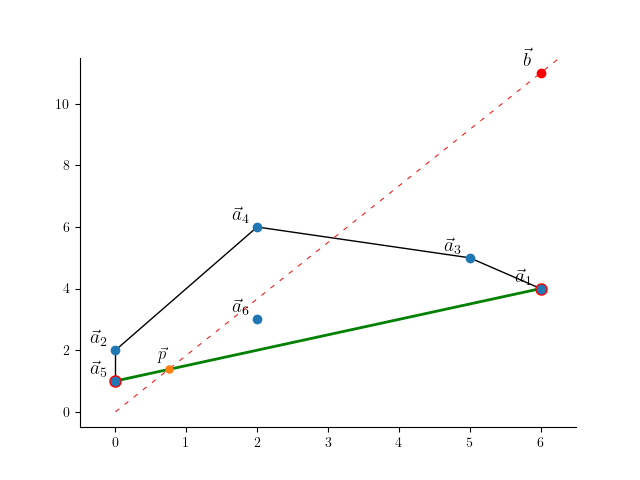
\includegraphics[height=5cm]{walkthrough_basis_selection.png}
    \caption{\label{fig:walkthrough_basis_selection} Geometrical basis selection for the example in this chapter.}
\end{figure}
When you take a look at figure \ref{fig:walkthrough_basis_selection}, it is clear that the corners of the facet that got hit first by the ray to $\vec b$ are $\vec a_1 = (6, 4)^\top$ and $\vec a_5 = (0, 1)^\top$ and hence
$$A' := (\vec a_1, \vec a_5) = \mat{6&0\\4&1} \quad \Rightarrow \Delta(A') = \mat{6-0&4-1} = \mat{6&3}$$
Low let us perform the second step of the algorithm. It is easy to see that $\solspace(\Delta(A'), \vec 0) = \Span\smat{-1\\2}$ and because $\det A'^\top = 6 \neq 0$ we know that $\solspace(A'^\top, \vec 0) = \{\vec 0\}$ and we can thus choose $\vec\mu = \smat{-1\\2}$. (And also $\sprod{\vec\mu}{\vec a_1} = 2 > 0$)

Now we have to convert the $\vec\mu$ we found into the correct Gauss elimination steps $C$, so that $A' := C\cdot A$ is our optimized matrix. (Note: Here we are reusing the symbol $A'$ for a different purpose.) We do this according to lemma \ref{lemma:construct_gauss_steps}:
$$D := \mat{-1&0\\0&2} \quad\Rightarrow \tilde A = D \cdot A = \mat{-6&0&-5&-2&0&-2\\8&4&10&12&2&6}$$
To construct $C'$, we set $c := \max_{i\in[2], j\in[6]}|\tilde A_{ij}| = 12$ and thus:
$$C' = \imat_2 + \opmat_2(c) = \mat{13&12\\12&13} \quad\Rightarrow C = C'\cdot D = \mat{-13&24\\-12&26}$$
$$A' = C \cdot A = \mat{18&48&55&118&24&46\\32&52&70&132&26&54}\qquad \vec b' = C\cdot \vec b = \mat{186\\214}$$
This is our optimised $A$. With this we can now do the construction from the theorem \ref{theorem:column_sum_construction} again. Let $s'_j$ be the $j$-th column sum of $A'$. $\alpha' = \max\{s'_1, \dots, s'_6\} = 118+132=250$, $v_j = \alpha - s_j$. Now let us define $k'$ and with it $\beta'$:

$$k' \geq \frac{1}{\min\{s'_1, \dots, s'_6\}} \sum_{i=1}^{2}b'_i = \frac{1}{24+26}(186+214) = 8 \quad \Rightarrow k' := 8$$ 
$$\beta' = k'\cdot\alpha' - \sum_{i=1}^{2}b'_i = 8\cdot250-(186+214) = 1600$$
This gives us the extended CCS ILP $(A'_{ext}, \vec b'_{ext}, \vec\omega'_{ext})$:
$$A'_{ext} = \mat{18&48&55&118&24&46&0\\32&52&70&132&26&54&0\\200&150&125&0&200&150&250}\quad\vec b':= \mat{186\\214\\1600}\quad \vec\omega'_{ext} = (1, 2, 3, 4, 5, 6, 0)^\top$$

Using this method, we have reduced the depth of the tree, in other words the number of layers, from $k=17$ to $k'=8$, resulting in a much smaller graph. If we also apply the graph optimisations discussed in chapter \ref{chap:graph_optimisation} and remove the childless vertices, we can see the final graph in figure \ref{fig:walkthrough_final_graph}.
\begin{figure}
    \centering
    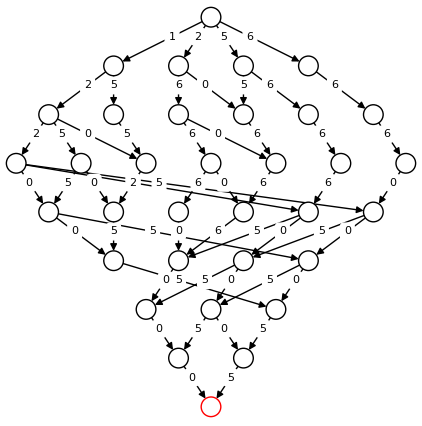
\includegraphics[height=6.5cm]{walkthrough_final_graph.png}
    \caption{\label{fig:walkthrough_final_graph} Graph constructed of $A'_{ext}, \vec b'_{ext}$. Vertex values are hidden.}
\end{figure}

\subsection{Discussion on slack variables}
It is common for an ILP to be given in its standard form. In order to be able to use the proposed algorithm, it must first be converted to slack form. As described in the observation \ref{obs:lp_slack_form}, we will extend $A$ by an identity matrix.

This has a huge impact on the results we can expect from the algorithm. Let us think about it: Since all unit vectors are present as column vectors of $A$, they will affect the convex hull. More precisely, all these unit vectors lie on the hyperplane $x_1 + \dots + x_n = 1$, and since no point can lie between the origin and this plane, this hyperplane will manifest itself as a facet of the convex hull. It is geometrically clear that any ray cast from the origin to any point $\vec b$ will always hit this plane first. Consequently, this surface will be selected by the algorithm, which means that the selected basis will be the standard basis.

So $A'$ will be some column permutation of the identity matrix. It is easy to see that $\Delta(A')\opvec(1) = \vec 0$ and $A'^\top\opvec(1) = \opvec(1) \neq \vec0$. Thus the algorithm could choose $\vec\mu = \opvec(1)$.

Why is this a problem now? $\opvec(1)$ represents the matrix $A$ itself without any modifications. And since the algorithm spits out the best possible matrix, we cannot improve $A$ any further.

So any ILP given in its standard form is solvable within the shortest path framework, but the execution cannot be improved.